% Pittsburgh 311 routing: final report
% Compile with pdfLaTeX (Overleaf default). No external files needed.
\documentclass[11pt,letterpaper]{article}

\usepackage[T1]{fontenc}
\usepackage[utf8]{inputenc}
\usepackage{mathptmx}
\usepackage[scaled=.90]{helvet}
\usepackage{microtype}
\usepackage[margin=1in]{geometry}
\usepackage{booktabs}
\usepackage{tabularx}
\usepackage{array}
\usepackage{caption}
\usepackage{titlesec}
\usepackage{enumitem}
\usepackage[hidelinks]{hyperref}
\usepackage{tikz}
\usetikzlibrary{positioning,arrows.meta,calc}
\usepackage{pgfplots}
\pgfplotsset{compat=1.17}

\setlength{\parindent}{0pt}
\setlength{\parskip}{0.7em}
\linespread{1.08}

\titleformat{\section}{\Large\bfseries\sffamily}{\thesection}{0.6em}{}
\titleformat{\subsection}{\large\bfseries\sffamily}{\thesubsection}{0.6em}{}
\titlespacing*{\section}{0pt}{1.6em}{0.4em}
\titlespacing*{\subsection}{0pt}{1.2em}{0.2em}

\captionsetup{font=small,labelfont=bf,labelsep=period,justification=raggedright,singlelinecheck=false,skip=6pt}
\renewcommand{\arraystretch}{1.18}
\newcolumntype{L}{>{\raggedright\arraybackslash}X}

\title{\sffamily\bfseries Can a Small Local Model Route Pittsburgh 311\\Requests Correctly on the First Try?}
\author{%
  Afaq Khan, Rizaldy Utomo, Mahika Gunjkar, and Ming-Chin Lu\\[0.4em]
  Carnegie Mellon University\\
  95-820 Applications of NL(X) and LLM \,|\, Group 3%
}
\date{Research Report \,|\, October 8, 2026}

\begin{document}

\maketitle

\begin{abstract}
\noindent Misclassified service requests require extra work from city staff and may take longer to reach the correct department. We examined whether a small local language model could help Pittsburgh 311 correctly classify requests, ask for missing information, and route them to the appropriate department on the first attempt. We combined the four team members' corpora, totaling 854 records, with official routing information and historical time-to-close statistics for 127 issue types. Using Phi-4-mini-instruct, we tested five approaches on the same 50 held-out inputs: a prompt-only baseline, retrieval, retrieval with codebook tools and neighbor voting, that approach with a safety guardrail, and LoRA fine-tuning. The best-performing approach correctly identified both the category and department for 41 of 50 inputs, achieving 82\% routing accuracy (95\% bootstrap confidence interval: 70\% to 92\%). The prompt-only baseline achieved 0\%, while LoRA fine-tuning reached 50\%. However, the best approach identified the specific issue correctly in only 60\% of cases, and its routing accuracy fell to 62\% on the 13 free-text complaints. This suggests that the overall score may overestimate performance on realistic resident submissions. The keyword-based guardrail maintained routing accuracy on non-adversarial inputs, but attack-blocking rates ranged from 42\% to 100\% across the three probe sets. These results support further development of a routing assistant with staff review. However, testing with city staff is needed to determine whether it can reduce request resolution time.
\end{abstract}

%------------------------------------------------------------
\section{Introduction}

Pittsburgh 311 handles non-emergency service requests related to streets, waste, buildings, parks, and other public infrastructure. Residents and staff need to match descriptions of these problems to the City's official categories and responsible departments. According to the City's data user guide, residents incorrectly classify about 5\% to 10\% of online submissions. Requests sent to the wrong department must then be reclassified and redirected by 311 staff~\cite{wprdc}. This historical estimate helps explain the need for better intake, but it does not reflect a measured error rate for the current system.

We examined whether an LLM-assisted intake and routing API could help reduce resolution time by improving how requests are handled at submission. We focused on four steps: classifying the complaint, identifying missing information, asking a targeted clarification question, and recommending the responsible department. We compared whether adding city-specific information improved routing over a prompt-only baseline, how retrieval and codebook tools performed against LoRA fine-tuning, and how the system handled realistic complaints and safety tests.

Our project produced a shared corpus covering four service domains, historical request-volume and closure-time statistics, and an integrated routing API. We evaluated five designs using the same test inputs and a reproducible evaluation process. We also analyzed performance by input type and documented guardrail failures to make the system's strengths and limitations clear. The API was developed as a research prototype for staff-reviewed routing recommendations and was not deployed in Pittsburgh's 311 system~\cite{team}.

%------------------------------------------------------------
\section{Related Works}

Our project compared retrieval, codebook tools, neighbor voting, guardrails, and LoRA fine-tuning using local Phi-4-mini-instruct. The team's individual experiments informed the integrated design. Ming-Chin's TF-IDF majority-voting approach informed the neighbor vote used in T2, while Mahika's category-definition experiments informed the guidance included in the knowledge cards. Rizaldy's LLMBox fork provided the API framework and guardrail, and Afaq's free-text complaints supplied the most realistic evaluation inputs~\cite{team}.

Across the individual experiments, official category definitions and department mappings helped the model produce more accurate labels. Structured output improved format consistency but did not guarantee correct predictions. These findings guided the team's comparison of five routing designs~\cite{team}.

The project developed in three rounds, shown in Figure~\ref{fig:iteration}. In Assignment 1, each member built a corpus and compared Phi-4-mini-instruct~\cite{phi4mini} against hand labels. The same failure appeared in every domain: the model usually recognized the topic but did not produce Pittsburgh's official labels. Department accuracy was 0\% at baseline in both the streets and parks corpora, where the model generated generic names such as ``Public Works'' and ``Parks and Recreation.'' In Assignment 2, each member built and evaluated an API that addressed this failure in a different way. The team design combined the approaches that worked best, and the final round evaluated it against a prompt-only baseline and a fine-tuned model~\cite{team}.

The individual experiments also compared Phi with larger hosted models, which bears directly on the choice of a small local model. On the streets corpus, Phi with Pittsburgh's routing rules in the prompt reached 40\% department accuracy, while Claude Sonnet without those rules reached 4\%, because it also defaulted to generic department names. On the waste corpus, GPT-5.6 Luna matched all three tags on 88\% of records against Phi's 36\%. Taken together, these comparisons suggest that model capability helps, but jurisdiction-specific knowledge matters more for the department field. A local model can use that knowledge without sending resident text to an outside provider~\cite{team}. Each comparison used 25 records and one prompt, so neither is a general benchmark.

\begin{figure}[htbp]
\centering
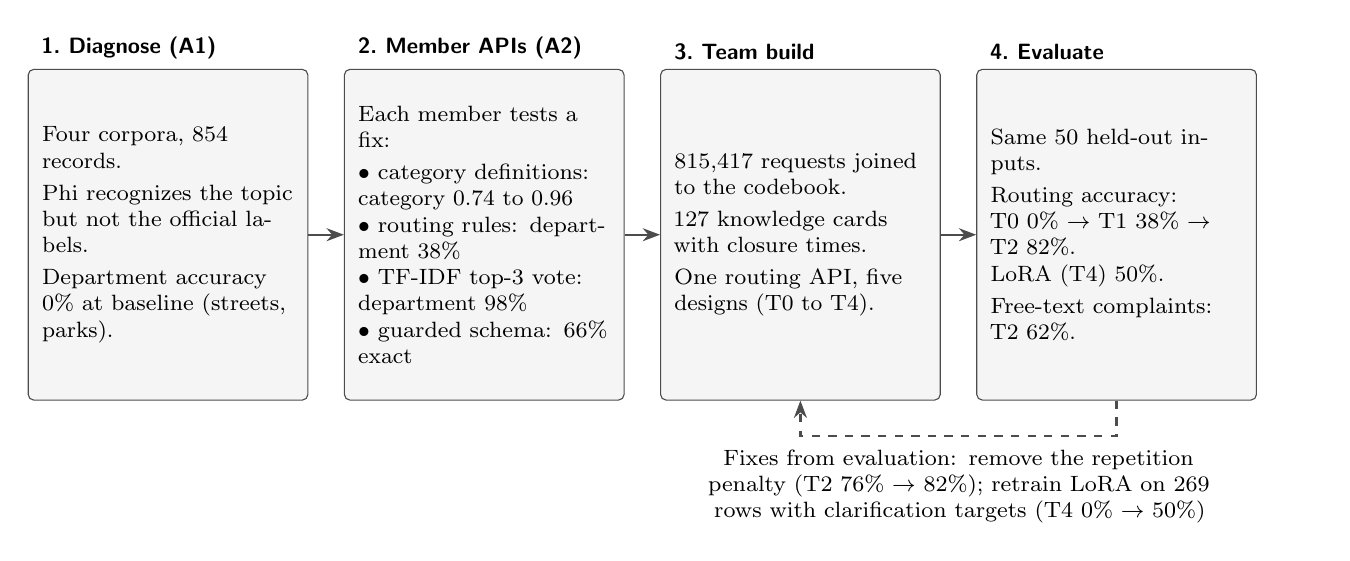
\begin{tikzpicture}[
  stage/.style={draw=black!70, rounded corners=2pt, fill=black!4, text width=3.2cm,
    align=left, font=\footnotesize, inner sep=5pt, minimum height=4.2cm, anchor=north},
  head/.style={font=\footnotesize\bfseries\sffamily, align=left, text width=3.2cm, anchor=south},
  arr/.style={-{Stealth[length=2.2mm]}, thick, black!70}]
\node[stage] (a1) at (0,0) {Four corpora, 854 records.\\[2pt]
  Phi recognizes the topic but not the official labels.\\[2pt]
  Department accuracy 0\% at baseline (streets, parks).};
\node[stage, right=0.45cm of a1] (a2) {Each member tests a fix:\\[2pt]
  $\bullet$ category definitions: category 0.74 to 0.96\\
  $\bullet$ routing rules: department 38\%\\
  $\bullet$ TF-IDF top-3 vote: department 98\%\\
  $\bullet$ guarded schema: 66\% exact};
\node[stage, right=0.45cm of a2] (tb) {815,417 requests joined to the codebook.\\[2pt]
  127 knowledge cards with closure times.\\[2pt]
  One routing API, five designs (T0 to T4).};
\node[stage, right=0.45cm of tb] (ev) {Same 50 held-out inputs.\\[2pt]
  Routing accuracy:\\
  T0 0\% $\to$ T1 38\% $\to$ T2 82\%.\\
  LoRA (T4) 50\%.\\[2pt]
  Free-text complaints: T2 62\%.};
\node[head] at (a1.north) {1.\ Diagnose (A1)};
\node[head] at (a2.north) {2.\ Member APIs (A2)};
\node[head] at (tb.north) {3.\ Team build};
\node[head] at (ev.north) {4.\ Evaluate};
\draw[arr] (a1.east) -- (a2.west);
\draw[arr] (a2.east) -- (tb.west);
\draw[arr] (tb.east) -- (ev.west);
\draw[arr, dashed] (ev.south) -- ++(0,-0.45) -| (tb.south);
\node[font=\footnotesize, align=center, text width=9cm, anchor=north]
  at ($(tb.south)!0.5!(ev.south) + (0,-0.5)$)
  {Fixes from evaluation: remove the repetition penalty (T2 76\% $\to$ 82\%);
   retrain LoRA on 269 rows with clarification targets (T4 0\% $\to$ 50\%)};
\end{tikzpicture}
\caption{How the project developed. Each round fixed a failure found in the round before; the dashed loop shows the two changes made after the first full evaluation. Numbers in rounds 1 and 2 come from each member's own data and metrics and are not comparable with the team evaluation in round 4~\cite{team}.}
\label{fig:iteration}
\end{figure}

%------------------------------------------------------------
\section{Methodology}

\subsection{Organizational task and data preparation}

The API reads a resident's complaint and returns a structured ticket containing the service domain, category, issue, responsible department, missing information, a clarification question, confidence score, abstention flag, and historical time-to-close range. The system predicts the domain from the complaint rather than receiving it as an input. The four domains cover the 17 official categories specified in the shared project brief~\cite{team}. Since team members built their corpora using different types of content, the combined dataset is not a consistently sampled set of resident requests.

\begin{table}[htbp]
\centering
\caption{Member corpora used to construct the shared knowledge base~\cite{archive}.}
\label{tab:corpora}
\begin{tabularx}{\textwidth}{@{}l l r L@{}}
\toprule
Domain & Lead & \multicolumn{1}{c}{$n$} & Content \\
\midrule
Streets and mobility & Afaq Khan & 190 & Historical requests, resident-style complaints, routing cards \\
Waste and cleanliness & Rizaldy Utomo & 180 & Official guidance, codebook rows, summaries \\
Buildings and accessibility & Mahika Gunjkar & 260 & Requests with text and structured fields \\
Parks and public facilities & Ming-Chin Lu & 224 & Examples and closure records for 28 issues \\
\bottomrule
\end{tabularx}
\end{table}

The WPRDC archive snapshot used in our study contained 815,417 requests~\cite{team,archive}. We read request type IDs as strings, removed codebook entries with blank categories, and kept the latest codebook version for each ID. We then linked the requests to the codebook using a many-to-one left join. Of the total requests, 612,222 fell within our four service domains, 142,060 could not be matched to a category, and 61,135 belonged to categories outside our scope. These figures describe the historical data covered by the study, not the number of records used to train the model.

\subsection{Knowledge and routing architecture}

We combined the 854 corpus records and created 127 issue knowledge cards. Each card includes the official issue name, category, department, aliases, required information, and a clarification question written by the team. We also added historical closure statistics. After excluding intake examples, the knowledge-document index contained 397 documents. Labeled development examples were stored separately for retrieving similar requests~\cite{team}.

The retriever uses TF-IDF with lowercase text, English stop-word removal, unigram and bigram features, and sublinear term frequency. It measures similarity using dot products of normalized TF-IDF vectors. T1 includes three retrieved knowledge documents in the prompt. T2 includes three labeled development examples and ranks candidate issues using similarity-weighted votes from up to 25 development examples and issue cards among up to 25 retrieved knowledge documents. It then provides up to eight ranked candidates, along with exact issue-name matches from the codebook~\cite{team}.

After the model generates a response, T2 matches the approximate category and issues names to official labels and uses the corresponding knowledge card to assign the category and department. If the predicted issue cannot be matched, the system uses the highest-ranked issue from the vote. It also adds the card's clarification question when the output lists missing information but contains no question, and includes historical closure information when available. These rule-based steps are part of the evaluated pipeline, so the improvement in routing accuracy reflects the combined system rather than the LLM alone.

\begin{table}[htbp]
\centering
\caption{Five evaluated designs and their behavior changes~\cite{archive}.}
\label{tab:designs}
\begin{tabularx}{\textwidth}{@{}l L L@{}}
\toprule
Design & Information provided & Additional processing \\
\midrule
T0 & Complaint and allowed domains/categories & Prompt-only baseline \\
T1 & T0 plus three knowledge documents & Category normalization \\
T2 & Labeled neighbors, issue votes, codebook candidates & Issue normalization, card-based routing, vote fallback \\
T3 & Same routing context as T2 & Input guardrail and output redaction \\
T4 & Same short prompt as T0 on LoRA-adapted Phi & No retrieval or routing tools at inference \\
\bottomrule
\end{tabularx}
\end{table}

\subsection{Local model and adaptation}

We ran all final experiments locally on an Apple M4 using a Phi-4-mini-instruct with MPS acceleration and bfloat16 weights. All runs used greedy decoding, no repetition penalty, and a limit of 320 new tokens. We kept the base model and evaluation inputs the same across the five configurations to compare their performance under consistent conditions~\cite{team}.

For T4, we applied LoRA~\cite{lora} to the attention projection layers with rank 8 and alpha 16. The training set contained 269 development examples, with up to 80 from each domain and only 29 from waste. We trained for two epochs using AdamW, a learning rate of 0.0002, batch size 1, and gradient accumulation over four batches. The learning rate increased during three warmup steps and then decreased linearly, with gradient clipping set to 1.0. Training took approximately 30 minutes and completed 135 optimizer steps. For the 220 examples with matching knowledge cards, the training targets included clarification content from those cards~\cite{team}.

\subsection{Evaluation design and measures}

We extracted 584 intake examples from the team members' corpora. For building requests, we removed sentences that revealed the routing result or case status. We rewrote waste codebook entries as ``Resident reports: \textless issue\textgreater.'' These inputs no longer contain structured codebook fields, but they still name the issue directly, making them easier to classify than natural complaints. Using random seed 952 and stratification by member corpus, we split the data into 534 development examples and 50 evaluation examples~\cite{team}.

The evaluation set included 13 examples from the streets corpus, 12 from waste, 12 from buildings, and 13 from parks. After checking the labels against the codebook, the reference domains were streets (13), waste (12), buildings (11), and parks (14). Across the full dataset, 37 examples belonged to a different domain under the codebook than under their source corpus. This accounts for the difference between the source-corpus counts and the reference-domain counts.

Where possible, we matched request type IDs or issue names to the codebook to obtain reference labels for the issue, category, and department. Of the 50 evaluation examples, 36 used codebook labels and 14 retained team-member labels, including eight streets examples. Our leakage check found no matching evaluation IDs or texts in the 397-document knowledge index or the 534 development examples. This confirms that there was no direct overlap under the implemented check, although similar templates or wording may still appear across the datasets~\cite{team}.

Our primary metric, routing accuracy, counts a prediction as correct when both its category and department match the reference labels. The specific issue does not need to match. We also measured issue, department, domain, and category accuracy separately. Before comparing category and department names, we removed leading and trailing spaces and standardized capitalization. For issue names, we also removed the legacy ``DO NOT USE'' suffix. These separate measures matter because different issues can share a category and department.

We used the repository's 95\% percentile bootstrap confidence intervals, calculated from 1,000 resamples with seed 952. These intervals reflect uncertainty in the observed 50-example sample. Since T0 failed on all 50 examples, every bootstrap resample also produced zero accuracy, resulting in a 0\% to 0\% interval. This does not mean its true accuracy across all possible requests is exactly zero. We did not conduct paired significance tests between configurations.

We also measured Ticket311 schema validity, field completeness, clarification rate, abstention rate, generation latency, token counts, and accuracy by subgroup. Completeness indicates whether the domain, category, issue, and department fields contain values; it does not confirm that the ticket includes all information needed to handle the request. Similarly, clarification rate records whether a question was provided, not whether it was useful. We did not evaluate whether confidence scores reliably reflected prediction accuracy or whether the system abstained in appropriate cases.

\subsection{Safety and historical closure analysis}

T3 checks input text for known prompt-injection patterns, toxic content, and requests for system information. It also redacts selected content from the output. We tested the input filter using existing probe sets from three team members. These tests ran the filter without generating model responses, so the reported blocking rates measure filter decisions rather than the full system's resistance to attacks. None of the 50 routing evaluation inputs contained adversarial attacks~\cite{team}.

For the historical analysis, we calculated time to close by subtracting each request's creation timestamp from its closure timestamp and converting the result to days. We included only closed requests with valid dates and nonnegative durations, then calculated the median, 75th percentile, and 90th percentile for each issue. These figures describe historical administrative closure times. They do not measure actual repair times or show how the prototype would affect service resolution.

%------------------------------------------------------------
\section{Findings}

\subsection{Overall routing performance}

As shown in Table~\ref{tab:routing}, T2 and T3 correctly routed 41 of 50 inputs (82\%). T1 correctly routed 19 (38\%), T4 routed 25 (50\%), and T0 routed none. T2's routing accuracy was 44 percentage points higher than retrieval alone and 32 points higher than the tested LoRA configuration. These results show that the combined approach performed best on this test set, but they do not establish how much voting, prompting, or rule-based codebook lookup contributed individually~\cite{team}.

\begin{table}[htbp]
\centering
\caption{Accuracy and latency on the same 50 evaluation inputs~\cite{archive}.}
\label{tab:routing}
\begin{tabular}{@{}l r r l r@{}}
\toprule
Design & \multicolumn{1}{c}{Issue} & \multicolumn{1}{c}{Department} & Routing and 95\% CI & \multicolumn{1}{c}{Latency} \\
\midrule
T0 & 56\% & 0\%  & 0\% (0\% to 0\%)    & 11.9 s \\
T1 & 56\% & 70\% & 38\% (26\% to 52\%) & 15.2 s \\
T2 & 60\% & 82\% & 82\% (70\% to 92\%) & 15.0 s \\
T3 & 60\% & 82\% & 82\% (70\% to 92\%) & 18.5 s \\
T4 & 60\% & 58\% & 50\% (36\% to 64\%) & 9.4 s \\
\bottomrule
\end{tabular}
\end{table}

T0 correctly identified the issue in 56\% of cases but did not select the official department in any case. Its prompt listed the allowed categories without providing a routing table, so it generated plausible but generic department names such as ``Public Works.'' Adding retrieval increased department accuracy to 70\%, while T2's knowledge-card lookup raised it to 82\%. However, T2's specific issue accuracy was 60\%, showing that a ticket can reach the correct category and department even when its issue label is wrong.

Figure~\ref{fig:tradeoff} plots routing accuracy against generation time and prompt length. The two designs that use city knowledge take different routes to it. T2 puts the knowledge in the prompt at inference time, which roughly doubles the prompt (600 against 292 tokens) and reaches 82\%. T4 stores some of it in the adapter weights, keeps the short prompt, and is the fastest design at 9.4 seconds, but routes 50\% correctly. On this test set, retrieval and codebook grounding bought 32 points of routing accuracy for about 5.6 seconds of extra generation time per request.

\begin{figure}[htbp]
\centering
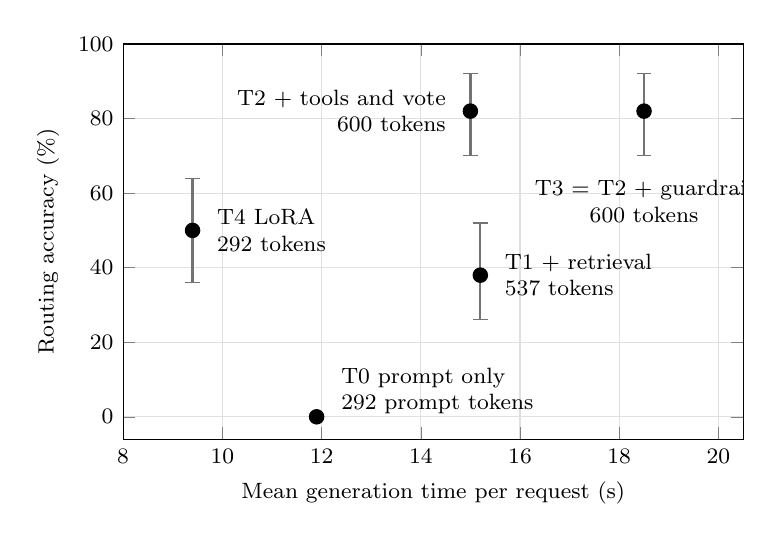
\begin{tikzpicture}
\begin{axis}[
  width=0.78\textwidth, height=6.6cm,
  xlabel={Mean generation time per request (s)},
  ylabel={Routing accuracy (\%)},
  xmin=8, xmax=20.5, ymin=-6, ymax=100,
  ytick={0,20,40,60,80,100},
  grid=major, grid style={black!12},
  tick label style={font=\footnotesize}, label style={font=\footnotesize},
  every node near coord/.append style={font=\footnotesize},
]
\addplot[only marks, mark=*, mark size=2.6pt, black,
  error bars/.cd, y dir=both, y explicit,
  error bar style={black!55, thick}]
  coordinates {
    (11.9,0)  +- (0,0)
    (15.2,38) -= (0,12) += (0,14)
    (15.0,82) -= (0,12) += (0,10)
    (18.5,82) -= (0,12) += (0,10)
    (9.4,50)  -= (0,14) += (0,14)
  };
\node[font=\footnotesize, anchor=west, align=left] at (axis cs:12.2,7) {T0 prompt only\\292 prompt tokens};
\node[font=\footnotesize, anchor=west, align=left] at (axis cs:15.5,38) {T1 + retrieval\\537 tokens};
\node[font=\footnotesize, anchor=east, align=right] at (axis cs:14.7,82) {T2 + tools and vote\\600 tokens};
\node[font=\footnotesize, anchor=north, align=center] at (axis cs:18.5,66) {T3 = T2 + guardrail\\600 tokens};
\node[font=\footnotesize, anchor=west, align=left] at (axis cs:9.7,50) {T4 LoRA\\292 tokens};
\end{axis}
\end{tikzpicture}
\caption{Accuracy against speed and prompt length on the same 50 inputs. Bars show 95\% bootstrap intervals. Generation time excludes retrieval and filtering, which run outside the model~\cite{team}.}
\label{fig:tradeoff}
\end{figure}

All five designs filled in the domain, category, issue, and department fields. Schema validity was 100\% for T0, T2, T3, and T4, and 98\% for T1. Clarification rates were 88\% for T0, 94\% for T1, 100\% for T2 and T3, and 86\% for T4. None of the designs abstained on the non-adversarial evaluation inputs. This does not establish whether they would appropriately abstain on ambiguous or out-of-scope requests~\cite{team}.

\subsection{Performance depends on input type}

\begin{table}[htbp]
\centering
\caption{Routing performance by input origin~\cite{archive}.}
\label{tab:inputtype}
\begin{tabular}{@{}l r r r@{}}
\toprule
Input type & \multicolumn{1}{c}{$n$} & \multicolumn{1}{c}{T2 correct} & \multicolumn{1}{c}{T4 correct} \\
\midrule
Free-text complaints                    & 13 & 8/13 (62\%)   & 2/13 (15\%)  \\
Service requests and example texts      & 25 & 21/25 (84\%)  & 20/25 (80\%) \\
Codebook-derived rows naming the issue  & 12 & 12/12 (100\%) & 3/12 (25\%)  \\
\bottomrule
\end{tabular}
\end{table}

The free-text complaints are the closest examples in our dataset to actual resident submissions, although they were not collected from live intake during the study. T2 correctly routed 62\% of these 13 complaints, making this result more relevant to deployment planning than the overall 82\% score. However, input type and service domain vary together in this dataset, so wording alone cannot explain the performance difference.

By reference domain, T2 correctly routed 12 of 14 parks requests, 9 of 11 buildings requests, all 12 waste requests, and 8 of 13 streets requests. T4 correctly routed 12, 8, 3, and 2 requests in those domains, respectively. T2 identified the specific streets issue correctly in only 4 of 13 cases (31\%). In 14 of its 50 predictions (28\%), the system used the highest-ranked voted issue because the model's output could not be matched to a knowledge card. This fallback helped the pipeline return an official issue label, but these cases need further review to understand why the model did not select a valid candidate~\cite{team}.

\subsection{Safety performance}

T3 achieved the same routing accuracy as T2 on the non-adversarial evaluation set. Average generation time was about 15.0 seconds for T2 and 18.5 seconds for T3. This difference should not be attributed directly to the guardrail, because the recorded latency measures model generation time. We did not measure the filter's processing time separately.

\begin{table}[htbp]
\centering
\caption{Input guard decisions on member probe sets~\cite{archive}.}
\label{tab:guard}
\begin{tabular}{@{}l r r r r@{}}
\toprule
Probe origin & \multicolumn{1}{c}{Attack probes} & \multicolumn{1}{c}{Blocked} & \multicolumn{1}{c}{Benign probes} & \multicolumn{1}{c}{Passed} \\
\midrule
Mahika buildings & 16 & 16/16 (100\%) & 12 & 12/12 (100\%) \\
Rizaldy waste    & 14 & 12/14 (86\%)  & 16 & 15/16 (94\%)  \\
Ming-Chin parks  & 12 & 5/12 (42\%)   & 10 & 10/10 (100\%) \\
\bottomrule
\end{tabular}
\end{table}

Table~\ref{tab:guard} uses the attack and benign-input counts from the team's evaluation script. The script reclassifies some probes when standardizing the records, so these counts may differ from those reported in the individual memos. The filter blocked familiar attack patterns but missed many new or politely worded attacks in the parks set. It also blocked one legitimate waste input. These results show that the filter can both miss attacks and incorrectly block normal requests.

Team members' individual experiments also showed that malicious instructions embedded in corpus records could influence the model~\cite{team}. Retrieved content therefore needs to be treated as untrusted input. The team's probe tests evaluated only the input filter; they did not test the full pipeline against attacks in retrieved documents, information leaks in model outputs, or unauthorized tool actions.

\subsection{Historical operational baselines}

\begin{table}[htbp]
\centering
\caption{Historical closure statistics for the busiest issue in each domain~\cite{archive}. Durations are in days.}
\label{tab:closure}
\begin{tabular}{@{}l r r r r r@{}}
\toprule
Issue & \multicolumn{1}{c}{Requests} & \multicolumn{1}{c}{Closed used} & \multicolumn{1}{c}{Median} & \multicolumn{1}{c}{P75} & \multicolumn{1}{c}{P90} \\
\midrule
Potholes             & 65,666 & 65,233 & 10.1 & 31.9 & 86.8  \\
Weeds/Debris         & 77,513 & 65,928 & 19.9 & 48.9 & 128.1 \\
Building Maintenance & 28,863 & 22,209 & 28.8 & 97.1 & 383.9 \\
Overgrowth           & 10,771 & 10,536 & 21.6 & 63.9 & 161.1 \\
\bottomrule
\end{tabular}
\end{table}

Table~\ref{tab:closure} reports durations in days. Request counts include all records for each issue, while closure statistics include only closed requests with valid, nonnegative durations. The large gaps between the median and upper percentiles show that some requests took much longer to close, particularly those involving building maintenance. These figures provide historical context for intake recommendations, but they should not be used as promised completion times. Since open requests are excluded, the statistics may underrepresent cases with longer closure times.

\subsection{Development lessons}

Table~\ref{tab:iterations} lists the changes we made to the team pipeline in order. Most were found by reading raw model outputs rather than summary scores, and several fixed problems in the evaluation itself rather than in the model.

\begin{table}[htbp]
\centering
\caption{Changes made during development of the team pipeline, in order~\cite{team}.}
\label{tab:iterations}
\begin{tabularx}{\textwidth}{@{}L L L@{}}
\toprule
What we observed & What we changed & Effect \\
\midrule
Some inputs stated the answer (``It was routed to \ldots'') or were raw codebook rows & Removed routing and status sentences; rewrote codebook rows as ``Resident reports: \textless issue\textgreater.'' & Removes direct answer leakage; codebook rows still name the issue \\
Member labels disagreed with the codebook on 114 categories and 28 departments & Took gold labels from the codebook wherever an ID or issue name matched & 36 of 50 evaluation labels from the codebook \\
Phi paraphrased issue names and sometimes produced truncated JSON & Snapped issues to codebook names, fell back to the top voted issue, and salvaged fields from broken JSON & Development smoke test rose from 2 to 4 correct of 8 \\
With a repetition penalty of 1.15, the fine-tuned model left category and issue empty & Removed the penalty for every design & T0 issue 16\% $\to$ 56\%; T2 routing 76\% $\to$ 82\% \\
The first LoRA run (149 rows, one epoch, no clarification targets) never named a real department & 269 rows, two epochs, card-based clarification targets & Routing 0\% $\to$ 50\%; clarification 0\% $\to$ 86\% \\
The training framework stalled before its first step on the laptop GPU & Replaced it with a plain PyTorch training loop & Training completed in about 30 minutes \\
\bottomrule
\end{tabularx}
\end{table}

The repetition penalty may have discouraged copying official labels from the prompt, but we did not test this explanation separately. The two LoRA runs changed the data volume, epochs, and targets together, so their individual effects remain unclear. The first run's scores are recorded in the experiment README, but its response files were overwritten by the second run. Both comparisons therefore document development history rather than controlled ablations~\cite{team}.

%------------------------------------------------------------
\section{Discussion}

\subsection{Implications for municipal intake}

City-specific routing knowledge improved the prototype's performance. T0 identified 56\% of issues correctly but failed to select official departments. T2 addressed this gap by matching issues to departments through the codebook. Adoption would require an updated routing table, approved clarification questions, and staff review.

Better routing could reduce reassignments and follow-up, but closure times also depend on staffing, ownership, inspections, and field work. We did not measure review time, reassignment rates, resident satisfaction, or time savings. The results support a staff-reviewed pilot, but do not establish cost savings or faster resolution.

\subsection{Interpretation of adaptation and system quality}

T4 reached 50\% routing accuracy with the same short prompt as T0, which scored 0\%. Performance was stronger on parks and buildings than on waste and streets, possibly reflecting differences in training coverage and input style. Waste had only 29 training examples, but we did not test larger or more balanced datasets to separate these effects. We also did not test LoRA combined with retrieval.

T2 produced schema-valid tickets and clarification questions for every input. However, valid formatting does not guarantee correct or complete information, and a question is not necessarily useful. Effective intake requires the details staff need to handle the request, beyond valid JSON and a department assignment.

\subsection{Trade-offs of a small local model for policy use}

Accuracy was only one of the criteria we weighed. Table~\ref{tab:tradeoffs} compares the two designs that use city knowledge on the other things a city would care about.

\begin{table}[htbp]
\centering
\caption{Trade-offs between the grounded design and the fine-tuned design.}
\label{tab:tradeoffs}
\begin{tabularx}{\textwidth}{@{}l L L@{}}
\toprule
Consideration & T2: retrieval, tools, and vote & T4: LoRA fine-tuning \\
\midrule
Routing accuracy & 82\% (70\% to 92\%) & 50\% (36\% to 64\%) \\
Speed and prompt size & 15.0 s, 600 prompt tokens & 9.4 s, 292 prompt tokens \\
When a routing rule changes & Edit the knowledge card; no retraining & Rebuild training data, retrain (about 30 minutes on our laptop), and re-evaluate \\
Auditability & Each ticket comes from a named codebook card that staff can check & The department comes from the adapter weights, with no record to point to \\
Failure mode & Falls back to the top voted issue (28\% of inputs), which is always a real codebook issue & 15 of its 21 wrong departments are names that do not exist in the codebook, such as ``Police - Zone 1'' \\
\bottomrule
\end{tabularx}
\end{table}

Maintenance matters because the routing table does change. The streets archive spans the renaming of the Department of Public Works units to the Department of Mobility and Infrastructure, so the same work appears under two department names~\cite{team}. In T2, a change like this is an edit to a knowledge card that staff can review. In T4, it requires new training examples and a new evaluation. For a city, the grounded design is also easier to audit, because every recommendation can cite the card it came from.

Running a small model locally has its own costs and benefits. Complaints never leave the machine, and there is no per-request fee, which matters for text that may contain residents' names or addresses. The model fits on a laptop, but only just: inference ran comfortably on our 24~GB machine, while LoRA training needed about 11~GB of GPU memory and failed while other applications were open. The individual hosted-model comparisons suggest a larger model would help with format and category, but not with Pittsburgh's department names unless it is given the same routing knowledge. We did not measure dollar costs for the team pipeline. The members' individual analyses reached different conclusions, from a clear saving at city-wide volume for building requests to no saving for low-volume knowledge-base tagging. The economic case therefore depends on volume and on how long staff take to review each suggestion~\cite{team}.

\subsection{Limitations}

The small benchmark combines free-text complaints, examples, and codebook rows that name the issue directly. It does not reflect the mix or ambiguity of live submissions. Fourteen evaluation labels, including eight streets labels, rely on team-member judgment. Leakage checks exclude direct overlap but not semantic similarity, and the team reviewed the benchmark during development. A separate test set kept untouched until final evaluation would better assess generalization.

T2 combines several changes, so we cannot isolate the LLM's contribution without testing retrieval-only classification and separate voting and codebook components. Results are limited to one model, machine, and decoding setup. The bootstrap intervals do not account for label uncertainty, variation across runs, or differences from actual city operations.

Safety testing covered existing member probes and input-filter decisions. We did not validate confidence calibration or appropriate abstention. The historical archive stopped updating in 2025~\cite{archive}. Archived routing rules should be confirmed before operational use.

%------------------------------------------------------------
\section{Future Work}

We recommend testing the system on a larger set of de-identified resident complaints, with labels confirmed independently by city staff. The test set should include incomplete descriptions, typos, ownership questions, uncommon issues, and out-of-scope requests. It should remain separate from development, with results reported by domain and input style.

Further experiments should isolate the routing components by testing TF-IDF voting without the LLM, retrieval without fallback, and codebook lookup without voting. We would also test LoRA with retrieval and use more balanced training data. Results should distinguish raw model predictions from final tickets and report fallback rates alongside accuracy.

City staff should review whether the system identifies missing details and asks useful clarification questions. Confidence scores and referral thresholds also need evaluation. Safety testing should cover malicious retrieved records and reworded attacks, while checking how often normal complaints are incorrectly blocked.

Finally, a controlled pilot should compare the assistant with existing intake using reassignment rates, staff review time, follow-up frequency, and closure time. Staff should retain final routing authority, and each recommendation should record its supporting evidence and codebook version. This pilot would determine whether improved routing helps resolve requests faster.

%------------------------------------------------------------
\section{Conclusion}

On the 50-input test set, adding Pittsburgh's routing knowledge to Phi-4-mini increased category-and-department accuracy from 0\% to 82\%. LoRA fine-tuning alone reached 50\%. However, the best design achieved only 60\% issue accuracy and 62\% routing accuracy on free-text complaints. These results show both its improvement and its remaining limitations.

The system could help 311 staff review routing recommendations based on official city information. Further evaluation should focus on exact labels, realistic complaints, and security testing. The results do not establish readiness for operational use or faster resolution. Independent testing and a controlled pilot with city staff are needed before adoption.

%------------------------------------------------------------
\begin{thebibliography}{9}
\raggedright
\bibitem{wprdc} Western Pennsylvania Regional Data Center. (n.d.). \emph{City of Pittsburgh 311 Data User Guide}. \url{https://wiki.wprdc.org/wiki/City_of_Pittsburgh_311_Data_User_Guide}

\bibitem{team} Khan, A., Utomo, R., Gunjkar, M., \& Lu, M.-C. (2026). \emph{Pittsburgh 311 Municipal Service Resolution} [Course project repository]. Carnegie Mellon University, 95-820 Applications of NL(X) and LLM. \url{https://github.com/rzrizaldy/cmu_application_nlx_llm_team3}

\bibitem{phi4mini} Microsoft. (2025). \emph{Phi-4-Mini Technical Report: Compact yet Powerful Multimodal Language Models via Mixture-of-LoRAs}. arXiv:2503.01743. \url{https://arxiv.org/abs/2503.01743}

\bibitem{lora} Hu, E. J., Shen, Y., Wallis, P., Allen-Zhu, Z., Li, Y., Wang, S., Wang, L., \& Chen, W. (2022). LoRA: Low-rank adaptation of large language models. \emph{International Conference on Learning Representations}. \url{https://arxiv.org/abs/2106.09685}

\bibitem{archive} City of Pittsburgh. (n.d.). \emph{311 Data Archive} [Data set and issue/category codebook]. Western Pennsylvania Regional Data Center. \url{https://data.wprdc.org/dataset/311-data}
\end{thebibliography}

\end{document}
